\chapter{Oprawa i zdanie pracy}
\label{chap:printing}

Gotową pracę inżynierską należy wydrukować w kilku egzemplarzach i w odpowiedni sposób oprawić --- w zależności od miejsca przeznaczenia. O szczegółach przygotowania wersji archiwalnej można przeczytać na stronie wydziału\footnote{\url{http://weka.pwr.edu.pl/studenci/dyplomanci/przygotowanie-wersji-archiwalnej}}. 

Praca w wersji dla opiekuna i recenzenta może być wdrukowana zarówno jedno- jak i obustronnie (należy pamiętać o dostosowaniu układu tekstu do metody wydruku!), istotny jest odpowiedni sposób oprawy. Do jej wykonania (dwóch egzemplarzy) potrzebne będą:
\begin{itemize}
    \item gruba, przeźroczysta folia do bindowania A4 (na przód) --- 2 szt.;
    \item czarna okładka do bindowania A4 (na tył) --- 2 szt.;
    \item tekturka do pracy inżynierskiej, pobierana z dziekanatu --- 2 szt.;
    \item \textbf{niebieski}, wsuwany, prostokątny grzbiet zaciskowy do bindowania, dobrany do grubości pracy (patrz rysunek~\ref{fig:grzbiet}) --- 2 szt..
\end{itemize}
Wymienione wyżej materiały można kupić za kilka złotych w papierniczym lub w sklepie internetowym. Oprawę wykonuje się samemu, bez wykorzystania narzędzi. Oba egzemplarze (dla opiekuna i recenzenta), należy dostarczyć do mnie.

\begin{figure}
    \centering
    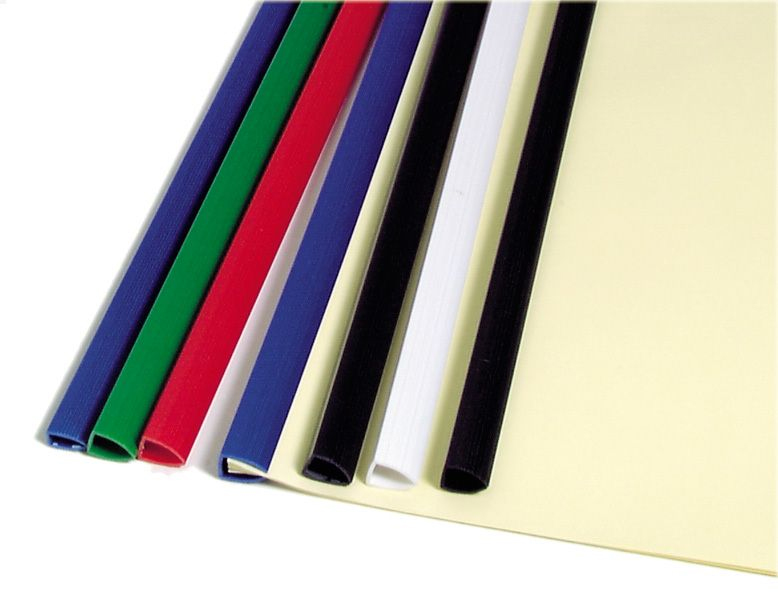
\includegraphics[width=\textwidth]{img/grzbiet.jpg}
    \caption{Grzbiety zaciskowe, do oprawy pracy dla promotora i recenzenta}
    \label{fig:grzbiet}
\end{figure}